\documentclass[a4paper]{article}

%% Language and font encodings
\usepackage[english]{babel}
\usepackage[utf8x]{inputenc}
\usepackage[T1]{fontenc}

%% Sets page size and margins
\usepackage[a4paper,top=3cm,bottom=2cm,left=3cm,right=3cm,marginparwidth=1.75cm]{geometry}

%% Useful packages
\usepackage{amsmath}
\usepackage{graphicx}
\usepackage[colorinlistoftodos]{todonotes}
\usepackage[colorlinks=true, allcolors=blue]{hyperref}

\title{Scribe Notes: Introduction to Weighted Bipartite Matching
August 24th 11:25am-12:00pm}
\author{Kelsey Sandlin}
\date{}  


\begin{document}
\maketitle

\section{Introduction to Weighted Bipartite Matching}

A \textbf{weighted bipartite graph} is a bipartite graph in which the edges between A and B have weights assigned to them. Example:
\begin{center}
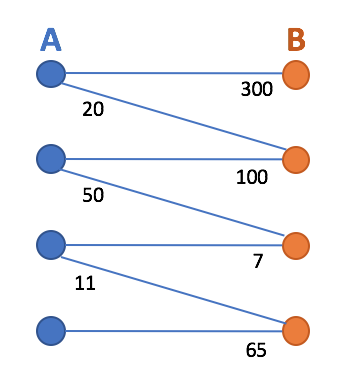
\includegraphics[width=4cm]{SampleWeighted.png}
\end{center}
Weighted Bipartite Graphs turn out to be more useful than bipartite graphs. 
The goal is to find a \textit{perfect matching*} that maximizes the weight:
\[max(\sum_{e\in M} w(e))\]

\subsection{A note on \textit{perfect matching*} in weighted bipartite graphs} 
There was a handful of student questions regarding selecting an \textit{imperfect} match to get a larger maximum of matched edge weights. 

In a weighted bipartite graph, one can always add zero-weight edges between points in A and points in B. Therefore if the solution is not a perfect matching, we can make it one at no additional cost by matching any un-matched pairs with zero-weight edges. For the examples today, you can  assume |A| = |B|.

\subsection{Realistic Examples}
Weighted bipartite graphs make are more useful for solving realistic problems than non-weighted bipartite graphs – you can think of set A as real estate sellers and set B as potential buyers where the edge weights are the prices of the houses. The sellers want to maximize profits, so the goal is to maximize matched edge weights:
	\[max(\sum_{e\in M} w(e))\]

You could also use set A to represent Jobs and set B to represent Workers – with the assumption that each worker can only perform one job. The goal is to finish all the jobs (therefore perfect matching is required) while minimizing the amount paid to the workers (matched edge weights):
	\[min(\sum_{e\in M} w(e))\]

\textbf{Aside: Are the maximization and minimization problems the same problem?}

Yes -- you can convert from maximization to minimization (or vice-versa) by multiplying the edge weights by -1:
	\[max(\sum_{e\in M} w(e)) = -min(\sum_{e\in M} -w(e))\]

\subsection{Introduction to the Algorithm}
How can we solve this problem to find the optimal perfect matching that maximizes edge weights?
\begin{itemize}
\item We will use some ideas about augmenting paths from the previous lecture
\item Apply the Alternating Path Algorithm, but only flip the path if the weight of the flipped version is greater than the current weight
\end{itemize}

This algorithm introduces the concept of a negative cycle.
A \textbf{Negative Cycle} is an alternating cycle that when flipped improves the weight.
In the below example a negative cycle, you can see that if you flip, you’ll get an increased total weight.
\begin{center}
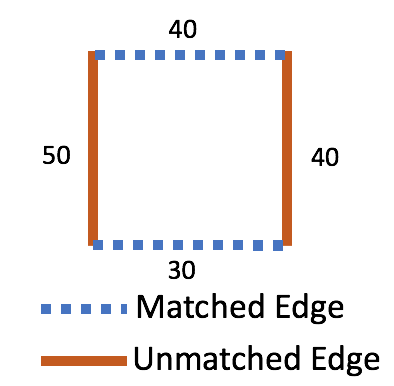
\includegraphics[width=4cm]{NegativeCycle.png}
\end{center}
Either there is a negative cycle in the graph, or you are at an optimal solution.


Unweighted Bipartite Matching Algorithm is O(mn) where m is number of edges and n is number of vertices. 

\textbf{Introduction to Kuhn-Munkres Algorithm: }
There might exist a more efficient algorithm based on Duality. This dual algorithm will deal with minimizing labels assigned to each vertex.


\end{document}